\documentclass[11pt,a4paper]{report}
\pdfoutput=1
\usepackage{inputenc}
\usepackage{fancyhdr,color}
\usepackage{amsfonts,amsmath,amssymb,graphics}
\usepackage[final]{pdfpages}
\usepackage{makeidx}
\makeindex
\usepackage{pdfpages}
\usepackage[pdftex,unicode=true,hyperfootnotes=false,colorlinks=true,citecolor=black,filecolor=black,linkcolor=black,urlcolor=black,pdfborder={0 0 0}]{hyperref}
\hypersetup{%
pdfstartview={Fit},%
pdftitle={Book},%
pdfauthor={Sciencesconf.org},%
pdfcreator={Sciencesconf.org},%
pdfproducer={PDFLaTeX - CCSD}
}
\urlstyle{same}
\pagestyle{plain}

\setlength{\topmargin}{0cm}
\setlength{\headheight}{0cm}
\setlength{\headsep}{0cm}
\setlength{\voffset}{-0.5cm}
\setlength{\textheight}{24.7cm}
\setlength{\textwidth}{16cm}
\setlength{\oddsidemargin}{0cm}
\setlength{\evensidemargin}{0cm}
\setlength{\parindent}{0.25in}
\setlength{\parskip}{0.25in}

\addtocontents{toc}{\protect\pagenumbering{roman}}

\lhead{}
\chead{}
\rhead{}
\lfoot{}
\cfoot{\thepage}
\rfoot{}

\renewcommand{\thefootnote}{\fnsymbol{footnote}}
\renewcommand{\contentsname}{Table of contents}
\renewcommand{\indexname}{Author Index}

\begin{document}

\newpage\thispagestyle{empty}
\topskip0pt
\par\vspace{2cm}
\begin{minipage}[l]{8cm}
\begin{center}
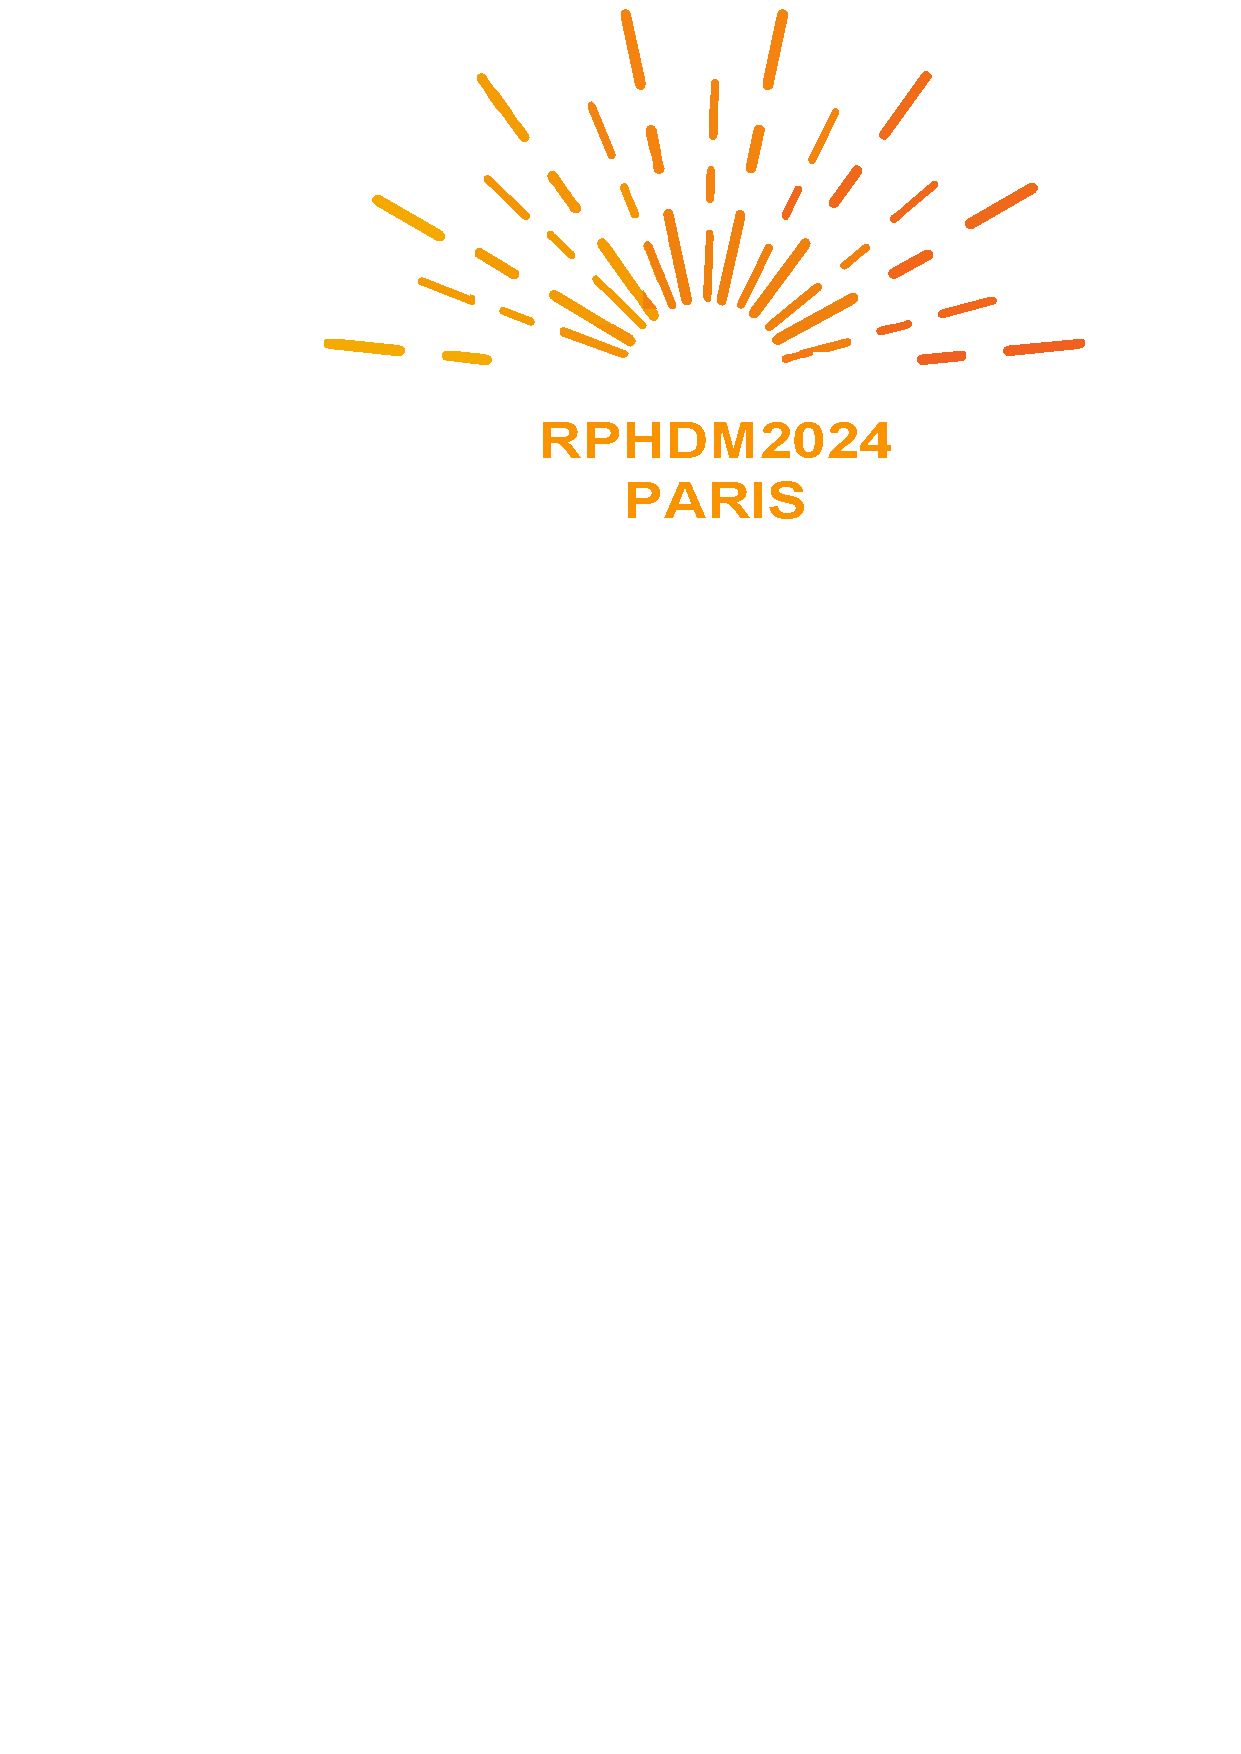
\includegraphics[scale=.5]{LOGO-RPHDM}\hspace{1.5cm}
\end{center}
\end{minipage}
\begin{minipage}[l]{9cm}
%\begin{center}
\begin{Large}
	\textcolor{blue}{{\Large {\bf 20th International Workshop on}}}
\par\vspace{.8cm}
	\textcolor{blue}{{\Large {\bf Radiative Properties}}}
\par\vspace{8mm}
\textcolor{blue}{{\Large {\bf 18-22 November 2024}}}
\par\vspace{8mm}
\par
\textcolor{blue}{{\Large {\bf Paris}}}
\end{Large}
%\end{center}
\end{minipage}\\
\par\vspace{5.cm}

\begin{center}
\begin{Huge}
\textbf{BOOK OF ABSTRACTS}
\end{Huge}\\
\par\vspace{7cm}
\end{center}

\newpage\thispagestyle{empty}
The RPHDM bi-annual meeting series started in 1984 and since 2000 it has been held alternating European and US locations. The last three editions took place in Santa Barbara, USA (2016), Hamburg, Germany (2018) and Santa Fe, USA (2022).

The purpose of the meeting is to bring together an international group of researchers studying radiation-dense matter interactions and related topics such as plasma spectroscopy, non-LTE population kinetics, opacity studies, spectral line shapes...


Covered topics

Previous meetings have covered hot-plasma absorption and emission spectroscopy, radiation heating, opacities, spectral line shapes, dense plasma effects and their role in the breakdown of the isolated atom model, non-equilibrium atomic kinetics and radiation transfer.

Experiments using high-intensity short-pulse lasers and z-pinch type discharges to generate and diagnose hot dense matter are central.  XUV, VUV and X-FEL sources, warm dense matter studies, and high-energy laser-related experiments, are particularly timely.



\newpage\thispagestyle{empty}
\begin{Large}
	{\bf SCIENTIFIC COMMITTEE}
\end{Large}

\noindent{\bf Jim Bailey}, Sandia, USA\\
{\bf Serena Bastiani}, LULI, Polytechnique, France\\
{\bf Djamel Benredjem}, LAC, Université Paris-Saclay, France\\
{\bf James Colgan}, Los Alamos National Laboratory, USA\\
{\bf Marta Fajardo}, Instituto Superior Tecnico, Lisboa, Portugal\\
{\bf Chris Fontes}, Los Alamos National Laboratory, USA\\
{\bf Carlos Iglesias}, Lawrence Livermore National Laboratory, USA\\
{\bf Roberto Mancini}, University of Nevada, Reno, USA\\
{\bf Jean-Christophe Pain}, CEA, France\\
{\bf Yuri Ralchenko}, NIST, Gaithersburg, USA\\
{\bf Evgeny Stambulchik}, Weizmann Institue of Science, Israel\\
{\bf Pedro Velarde}, Instituto de Fusion Nuclear GV, Spain\\
{\bf Feilu Wang}, National Astronomical Observatories, China\\
{\bf Justin Wark}, University of Oxford, UK\\
{\bf Hitoki Yoneda}, Institute for Laser Science, Japan\\
{\bf Beata Ziaja-Motyka}, CFEL, DESY, Germany
		
\par\vspace{.5cm}
\begin{Large}
	{\bf LOCAL ORGANIZING COMMITTEE}
\end{Large}

\noindent{\bf Djamel Benredjem}, LAC, Universit\'e Paris-Saclay (Chair)\\
{\bf Jean-Christophe Pain}, CEA (co-Chair)\\
{\bf Serena Bastiani}, LULI, Polytechnique\\
{\bf Christopher Bowen }, CEA\\
{\bf Olivier Guilbaud}, IJCLab, Universit\'e Paris-Sacaly\\
{\bf Sylvie Jacquemot}, LULI, Polytechnique\\
{\bf Patrick Renaudin}, CEA\\
{\bf Caterina Riconda}, LULI, Polytechnique\\
{\bf St\'ephane Sebban}, LOA, Polytechnique
		
\par\vspace{.5cm}
\begin{Large}
         {\bf SECRETARY}
\end{Large}

\hspace{1.cm} {\bf Ir\'ene Ratsimandresy}, Laboratoire Aimé Cotton





\newpage\thispagestyle{empty}
\begin{center}
\begin{Large}
         {\bf SPONSORS}
\end{Large}
\begin{itemize}
\item Laboratoire Aim\'e Cotton 
\item Universit\'e Paris-Saclay
\item CEA-DAM-DIF, France
\item Sorbonne Universit\'e, Paris
\end{itemize}
\includegraphics[scale=.5]{logoCNRS.jpg}\hspace{2cm}\includegraphics[scale=.1]{CEA_GB_logotype.png}\\
\par\vspace{.5cm}
\end{center}

\newpage\thispagestyle{empty}
\vspace*{\stretch{1}}
Laius histoire RPHDM

\begin{large}
	\noindent{\bf TOPICS}
\end{large}

$\bullet$ X-RAY SOURCES: XRS

$\bullet$ PLASMA SPECTROSCOPY

$\bullet$ WARM DENSE MATTER: WDM

$\bullet$ ASTROPHYSICAL PLASMAS: ASTRO

$\bullet$ MAGNETIC CONFINMENT FUSION: MCF

$\bullet$ SPECTRA LINE SHAPES: SLS

$\bullet$ INERTIAL CONFINMENT FUSION: ICF

$\bullet$ FREE ELECTRON LASERS: XFEL

The scientific program of the 2024 workshop consists of oral and poster contributions.

\vspace*{\stretch{1}}

\phantomsection\tableofcontents

\clearpage\phantomsection\addcontentsline{toc}{chapter}{\protect\numberline{}ATOMIC DATA AND PROCESSES. I}
\topskip0pt\vspace*{\fill}\begin{center}\begin{Large}\textbf{ATOMIC DATA AND PROCESSES. I}\end{Large}\end{center}\vspace*{\fill}

\pagenumbering{arabic}

\phantomsection\addcontentsline{toc}{section}{\protect\numberline{}{\bf ADP.I1}: NLTE-12, Benford’s Law for Atomic Databases and All That\\
\textit{\underline{Yu. Ralchenko}}}
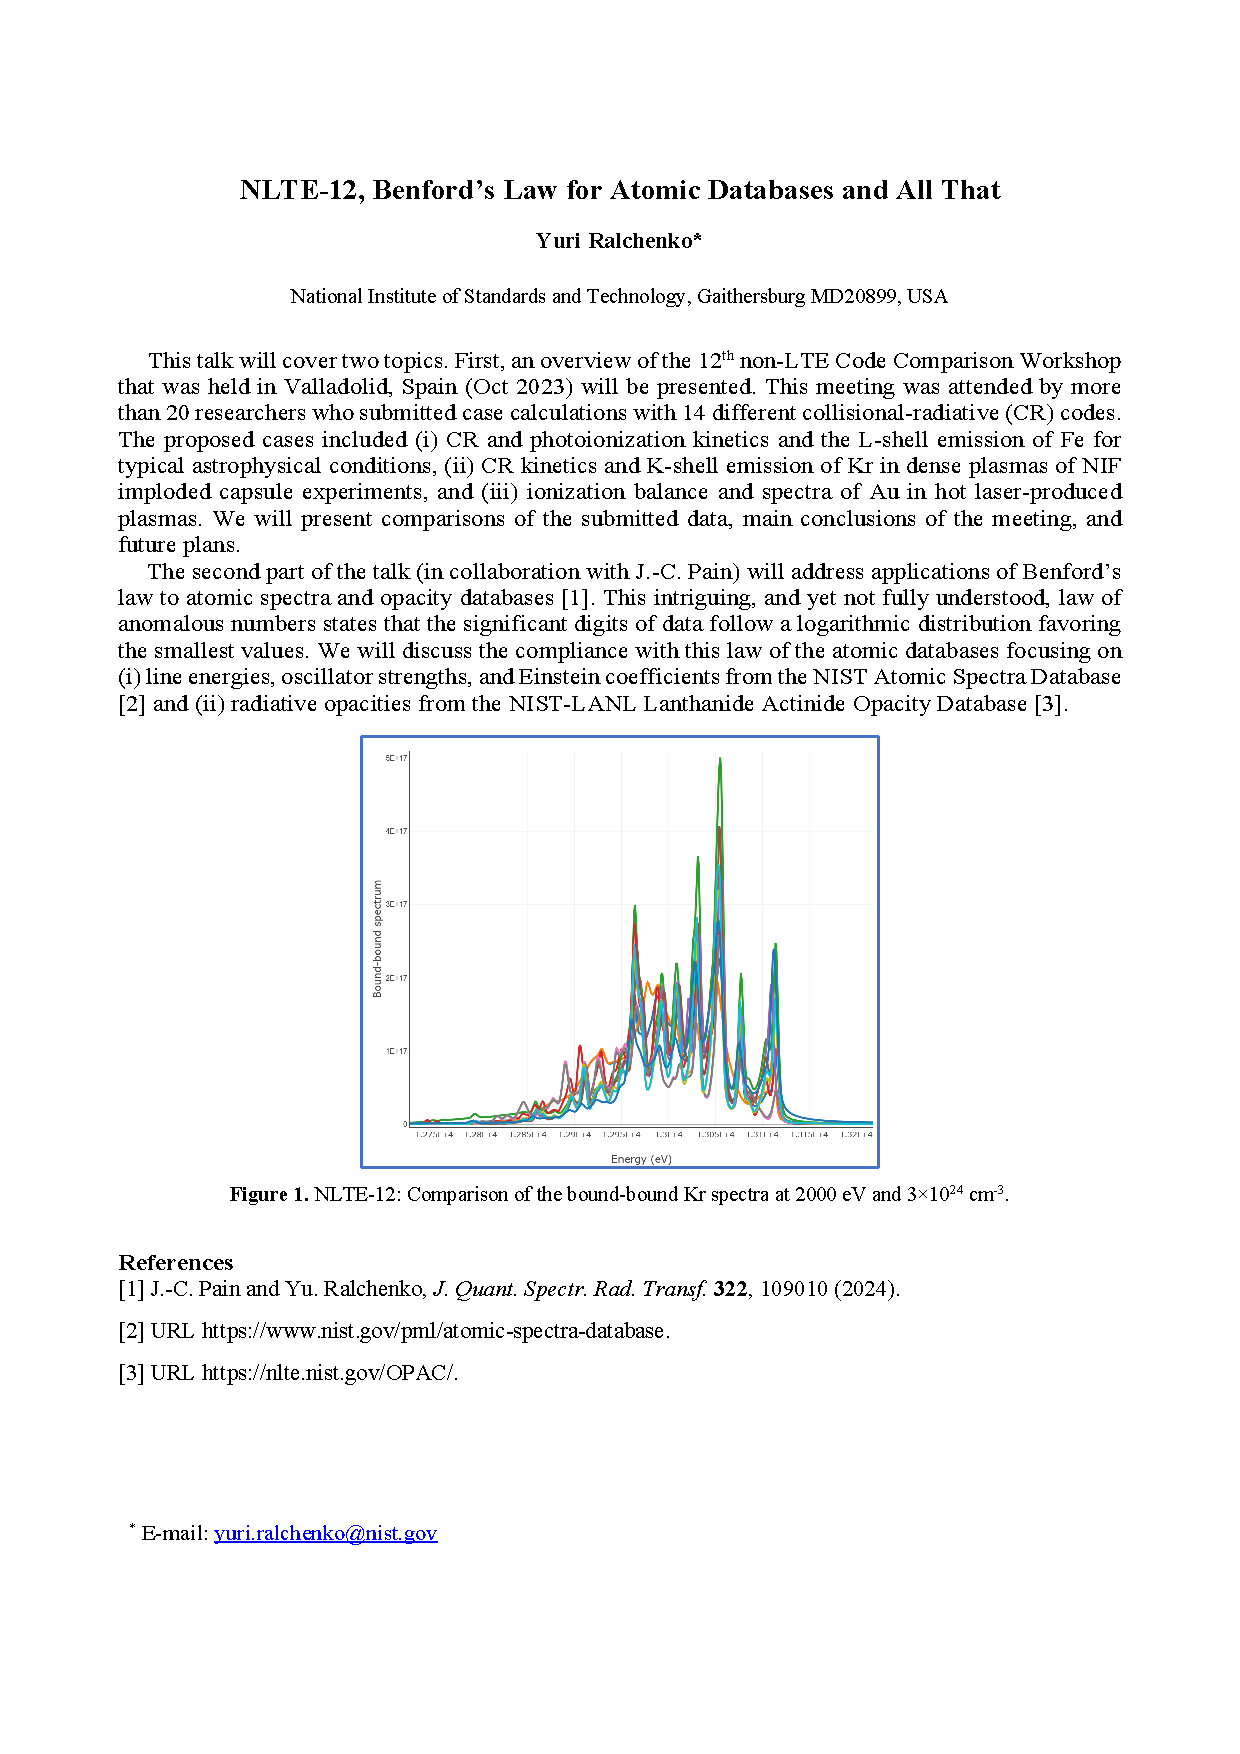
\includepdf[pages=-,pagecommand={\thispagestyle{fancy}\rfoot{\thepage}\cfoot{\bf \Large Invited}\index{Ralchenko Yu}}]{RALCHENKO.pdf}

\phantomsection\addcontentsline{toc}{section}{\protect\numberline{}{\bf ADP.I1}: Time-resolved spectroscopy for Z stellar opacity research\\
\textit{\underline{G. P. Loisel}}}
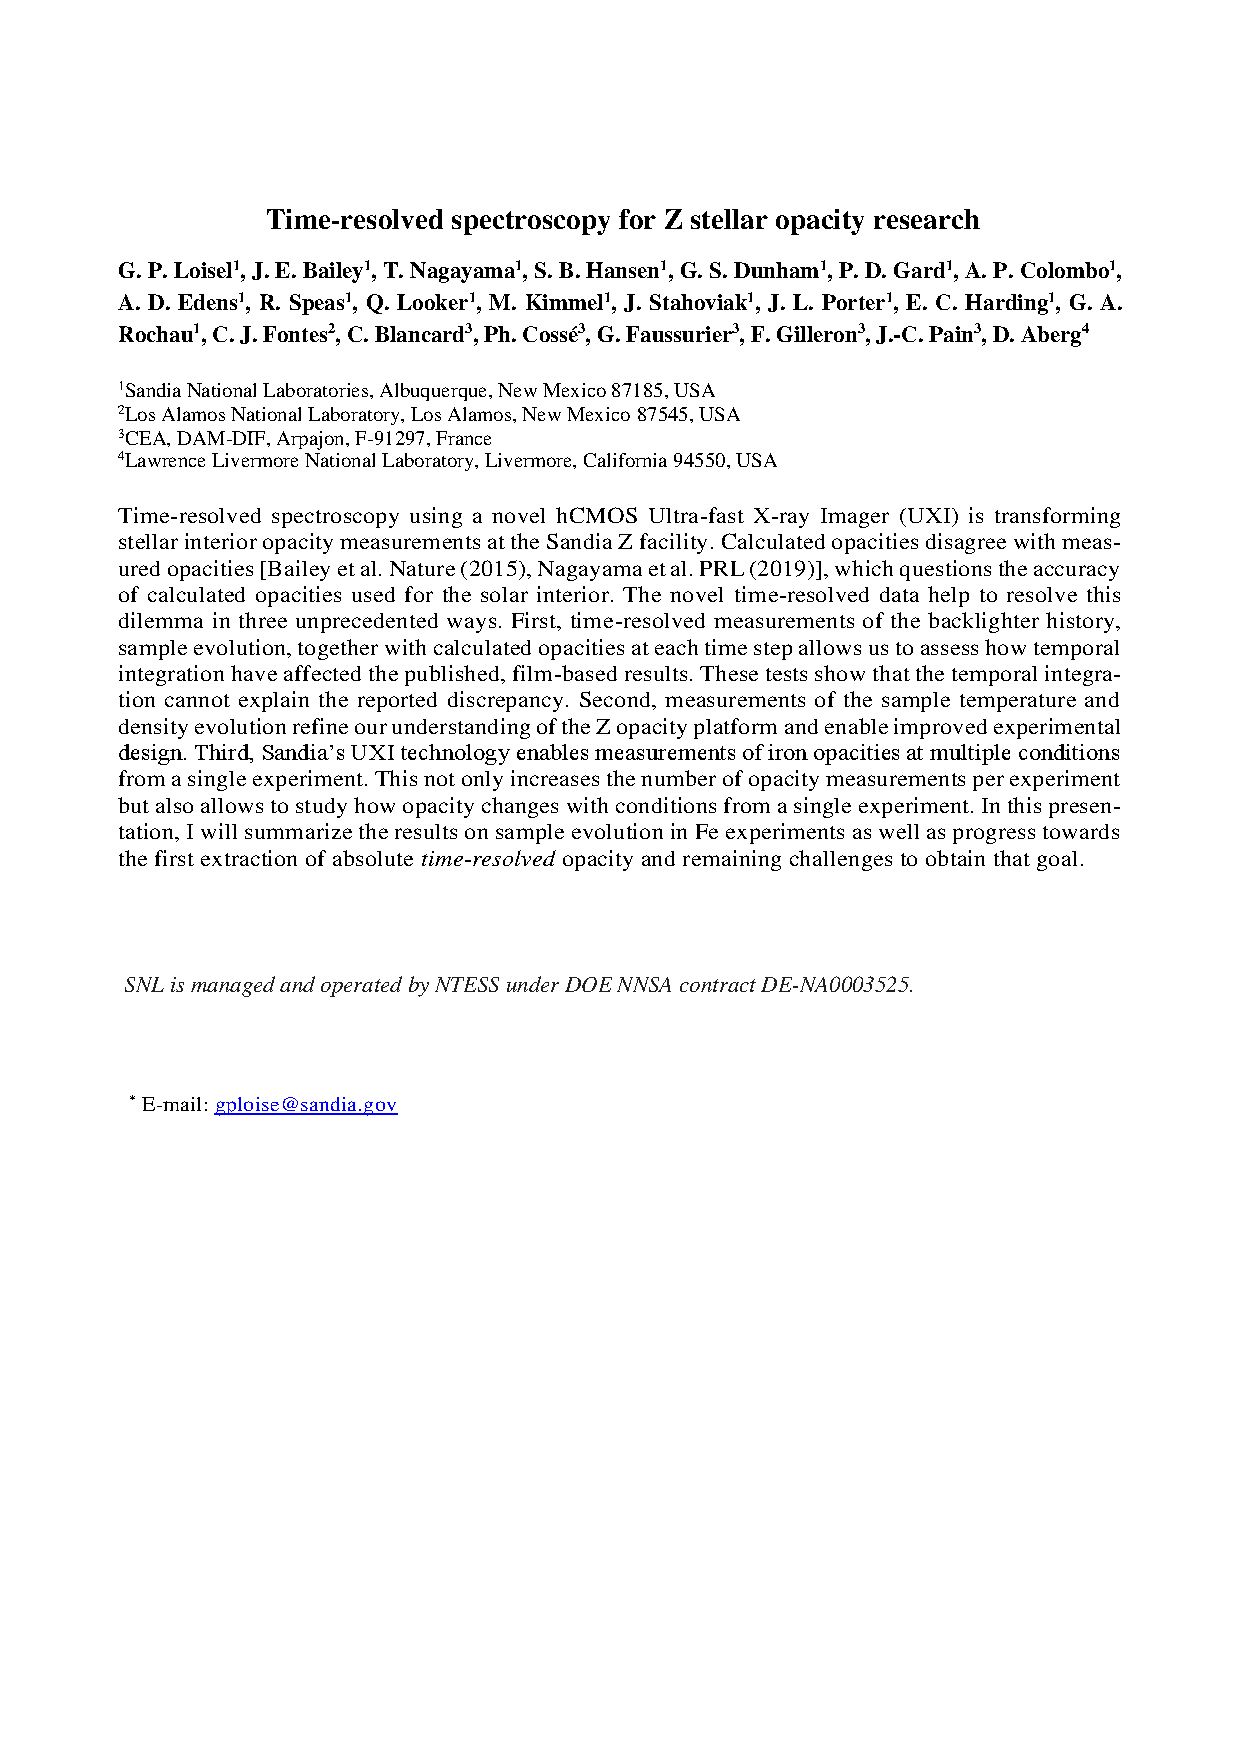
\includepdf[pages=-,pagecommand={\thispagestyle{fancy}\rfoot{\thepage}\cfoot{\bf \Large Invited}\index{Loisel G}}]{LOISEL.pdf}

\phantomsection\addcontentsline{toc}{section}{\protect\numberline{}{\bf ADP.I3}: Tungsten VUV spectroscopy in WEST tokamak 1-4 keV plasmas\\
\textit{\underline{R. Guirlet}}}
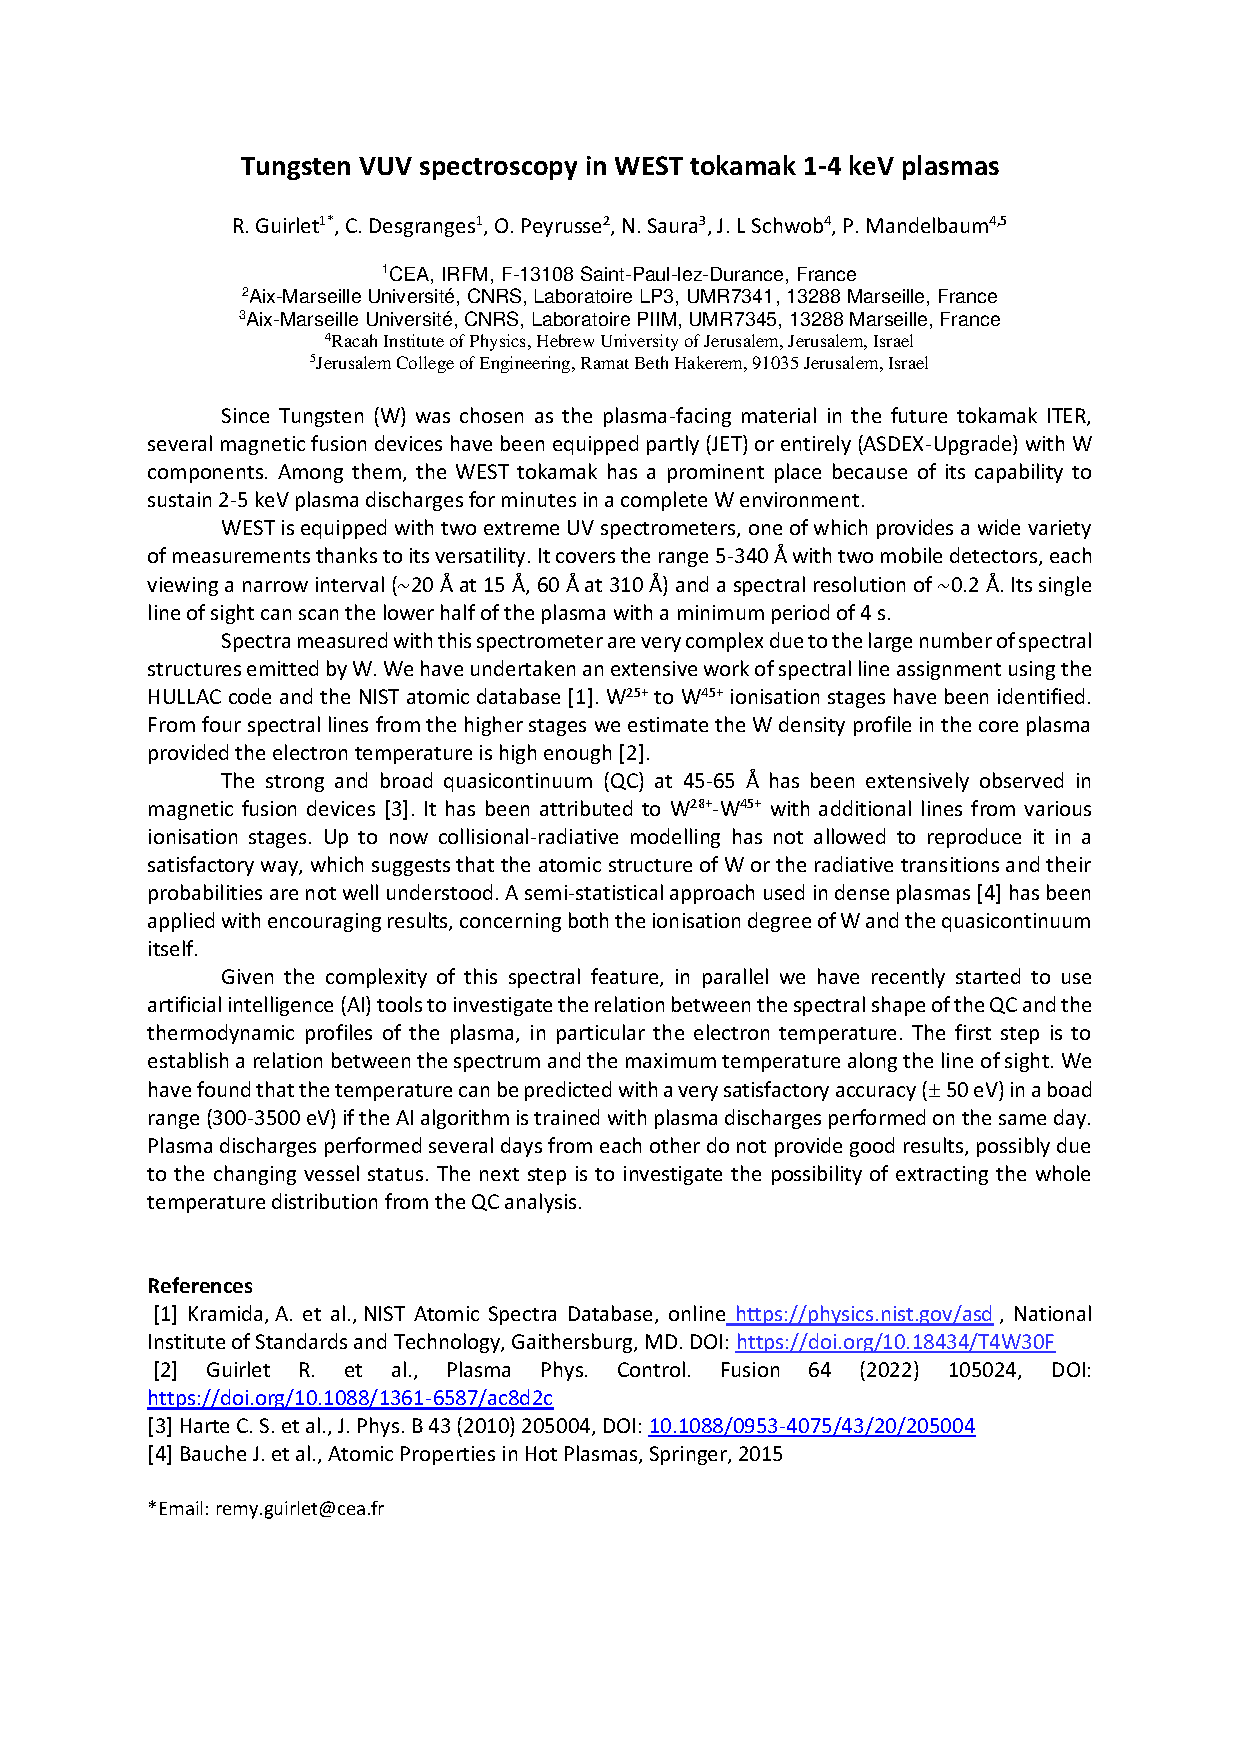
\includepdf[pages=-,pagecommand={\thispagestyle{fancy}\rfoot{\thepage}\cfoot{\bf \Large Invited}\index{Guirlet R}\index{Desgranges C}}]{GUIRLET.pdf}

\phantomsection\addcontentsline{toc}{section}{\protect\numberline{}{\bf ADP.I4}: High resolution, sub-picosecond x-ray spectroscopy of buried layers heated
with high intensity, short pulse lasers\\
\textit{\underline{R. Shepherd}}}
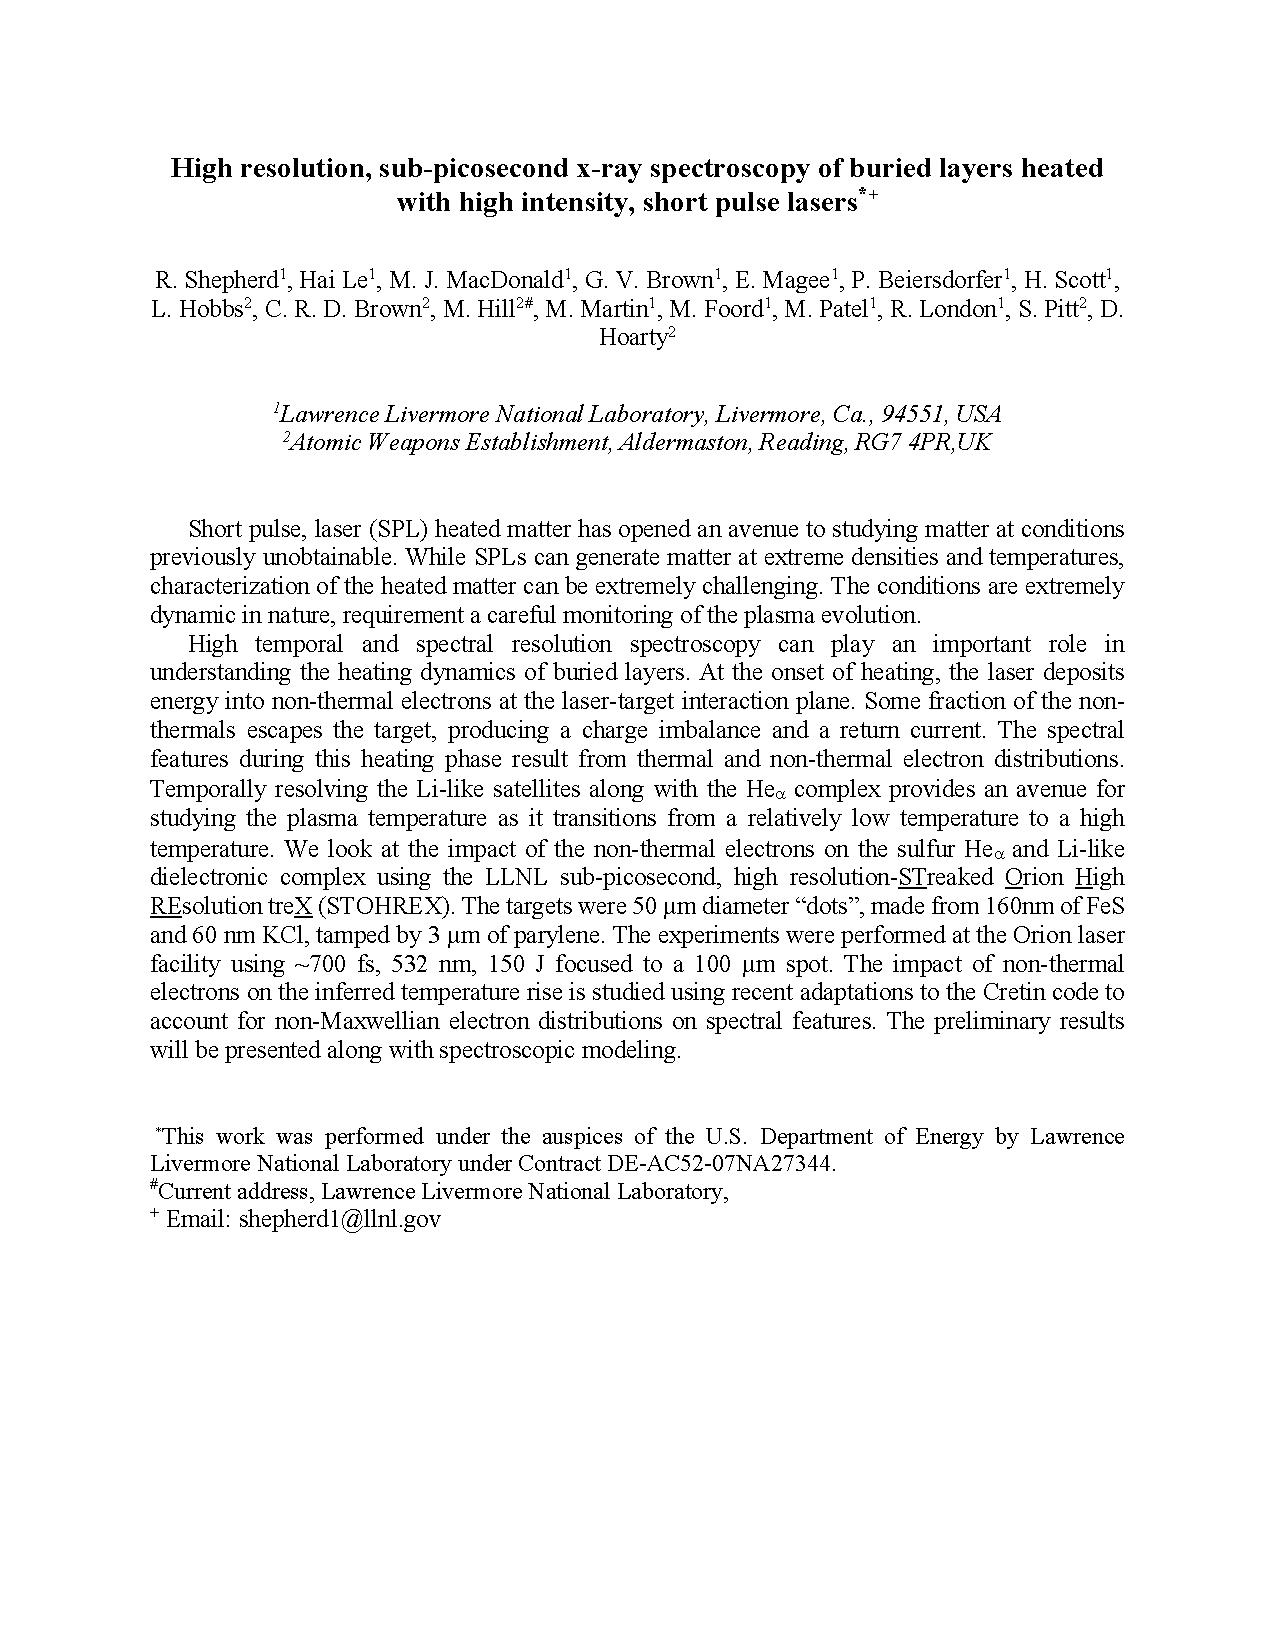
\includepdf[pages=-,pagecommand={\thispagestyle{fancy}\rfoot{\thepage}\cfoot{\bf \Large Invited}\index{Shepherd R}\index{Le H}}]{SHEPHERD.pdf}

\phantomsection\addcontentsline{toc}{chapter}{\protect\numberline{}Author Index}

\begin{theindex}

  \item Desgranges C, \hyperpage{4}

  \indexspace

  \item Guirlet R, \hyperpage{4}

  \indexspace

  \item Le H, \hyperpage{5}
  \item Loisel G, \hyperpage{3}

  \indexspace

  \item Ralchenko Yu, \hyperpage{2}

  \indexspace

  \item Shepherd R, \hyperpage{5}

\end{theindex}

\end{document}
